\newcommand{\gptpart}{8}
\newcommand{\gpttitle}{Defining the Break}
\newcommand{\gptsubtitle}{The Irreconcilable Differences Between General Relativity and Graviton Pressure Theory}
\newcommand{\gptdate}{November 2026}
% Shared preamble for the second edition of Graviton Pressure Theory.
% A part's own file sets \gptpart, \gpttitle, \gptsubtitle and \gptdate, then % Shared preamble for the second edition of Graviton Pressure Theory.
% A part's own file sets \gptpart, \gpttitle, \gptsubtitle and \gptdate, then % Shared preamble for the second edition of Graviton Pressure Theory.
% A part's own file sets \gptpart, \gpttitle, \gptsubtitle and \gptdate, then \input{../common/preamble}.
\documentclass[11pt,a4paper]{article}
\usepackage[T1]{fontenc}
\usepackage[utf8]{inputenc}
\usepackage{mathpazo}
\usepackage[scaled=0.92]{helvet}
\usepackage{amsmath,amssymb}
\usepackage[margin=2.5cm]{geometry}
\usepackage{microtype}
\usepackage{graphicx}
\usepackage{booktabs,array,tabularx}
\usepackage[font=small,labelfont=bf]{caption}
\usepackage{enumitem}
\usepackage[authoryear,round]{natbib}
\usepackage{titlesec}
\usepackage[titles]{tocloft}
\renewcommand{\cftsecfont}{\bfseries}\renewcommand{\cftsecpagefont}{\bfseries}
\renewcommand{\cftsecleader}{\hfill}\setlength{\cftsecnumwidth}{3.2em}
\usepackage{gpt-status}
\usepackage[hidelinks]{hyperref}
\setlength{\parskip}{4pt}
\setlength{\emergencystretch}{3em}
\setlength{\parindent}{0pt}
\setlist{itemsep=2pt,topsep=3pt}
\titleformat{\section}{\Large\bfseries}{\thesection}{1em}{}
\titleformat{\subsection}{\large\bfseries}{\thesubsection}{1em}{}
\renewcommand{\thesection}{\gptpart.\arabic{section}}
\renewcommand{\thetable}{\gptpart.\arabic{table}}
\renewcommand{\thefigure}{\gptpart.\arabic{figure}}
\renewcommand{\theequation}{\gptpart.\arabic{equation}}
\setcounter{tocdepth}{1}
\makeatletter\renewcommand{\@pnumwidth}{2.2em}\renewcommand{\@tocrmarg}{3em}
\makeatother
\bibliographystyle{plainnat}
\newcommand{\gptitle}{%
  \begin{titlepage}\centering
  \vspace*{3cm}
  {\Huge\bfseries Graviton Pressure Theory\par}\vspace{0.8cm}
  {\Large The Unified Framework\par}\vspace{0.2cm}
  {\large Individual Submission\par}\vspace{0.6cm}
  {\normalsize This document is part of a multi-part scientific framework\par}\vspace{2cm}
  {\normalsize Part \gptpart\ of 30\par}\vspace{0.8cm}
  {\huge\bfseries \gpttitle\par}\vspace{0.6cm}
  {\Large \gptsubtitle\par}\vspace{1.5cm}
  {\small\begin{minipage}{0.75\textwidth}\centering This submission is part of the broader Graviton Pressure Theory (GPT) project, a redefinition of gravitational interaction rooted in causal field dynamics and physical force transmission. Each document is designed to stand on its own; its full context emerges as part of the larger framework. For the complete series, see https://peopleoftheworld.net/graviton-pressure-theory/.\end{minipage}\par}
  \vfill
  {\large Author: Shareef Ali Rashada\par}\vspace{0.2cm}
  {\normalsize shareef@peopleoftheworld.net\par}\vspace{0.5cm}
  {\normalsize Second edition, \gptdate\par}
  \end{titlepage}
  \setcounter{page}{1}\tableofcontents\clearpage}
.
\documentclass[11pt,a4paper]{article}
\usepackage[T1]{fontenc}
\usepackage[utf8]{inputenc}
\usepackage{mathpazo}
\usepackage[scaled=0.92]{helvet}
\usepackage{amsmath,amssymb}
\usepackage[margin=2.5cm]{geometry}
\usepackage{microtype}
\usepackage{graphicx}
\usepackage{booktabs,array,tabularx}
\usepackage[font=small,labelfont=bf]{caption}
\usepackage{enumitem}
\usepackage[authoryear,round]{natbib}
\usepackage{titlesec}
\usepackage[titles]{tocloft}
\renewcommand{\cftsecfont}{\bfseries}\renewcommand{\cftsecpagefont}{\bfseries}
\renewcommand{\cftsecleader}{\hfill}\setlength{\cftsecnumwidth}{3.2em}
\usepackage{gpt-status}
\usepackage[hidelinks]{hyperref}
\setlength{\parskip}{4pt}
\setlength{\emergencystretch}{3em}
\setlength{\parindent}{0pt}
\setlist{itemsep=2pt,topsep=3pt}
\titleformat{\section}{\Large\bfseries}{\thesection}{1em}{}
\titleformat{\subsection}{\large\bfseries}{\thesubsection}{1em}{}
\renewcommand{\thesection}{\gptpart.\arabic{section}}
\renewcommand{\thetable}{\gptpart.\arabic{table}}
\renewcommand{\thefigure}{\gptpart.\arabic{figure}}
\renewcommand{\theequation}{\gptpart.\arabic{equation}}
\setcounter{tocdepth}{1}
\makeatletter\renewcommand{\@pnumwidth}{2.2em}\renewcommand{\@tocrmarg}{3em}
\makeatother
\bibliographystyle{plainnat}
\newcommand{\gptitle}{%
  \begin{titlepage}\centering
  \vspace*{3cm}
  {\Huge\bfseries Graviton Pressure Theory\par}\vspace{0.8cm}
  {\Large The Unified Framework\par}\vspace{0.2cm}
  {\large Individual Submission\par}\vspace{0.6cm}
  {\normalsize This document is part of a multi-part scientific framework\par}\vspace{2cm}
  {\normalsize Part \gptpart\ of 30\par}\vspace{0.8cm}
  {\huge\bfseries \gpttitle\par}\vspace{0.6cm}
  {\Large \gptsubtitle\par}\vspace{1.5cm}
  {\small\begin{minipage}{0.75\textwidth}\centering This submission is part of the broader Graviton Pressure Theory (GPT) project, a redefinition of gravitational interaction rooted in causal field dynamics and physical force transmission. Each document is designed to stand on its own; its full context emerges as part of the larger framework. For the complete series, see https://peopleoftheworld.net/graviton-pressure-theory/.\end{minipage}\par}
  \vfill
  {\large Author: Shareef Ali Rashada\par}\vspace{0.2cm}
  {\normalsize shareef@peopleoftheworld.net\par}\vspace{0.5cm}
  {\normalsize Second edition, \gptdate\par}
  \end{titlepage}
  \setcounter{page}{1}\tableofcontents\clearpage}
.
\documentclass[11pt,a4paper]{article}
\usepackage[T1]{fontenc}
\usepackage[utf8]{inputenc}
\usepackage{mathpazo}
\usepackage[scaled=0.92]{helvet}
\usepackage{amsmath,amssymb}
\usepackage[margin=2.5cm]{geometry}
\usepackage{microtype}
\usepackage{graphicx}
\usepackage{booktabs,array,tabularx}
\usepackage[font=small,labelfont=bf]{caption}
\usepackage{enumitem}
\usepackage[authoryear,round]{natbib}
\usepackage{titlesec}
\usepackage[titles]{tocloft}
\renewcommand{\cftsecfont}{\bfseries}\renewcommand{\cftsecpagefont}{\bfseries}
\renewcommand{\cftsecleader}{\hfill}\setlength{\cftsecnumwidth}{3.2em}
\usepackage{gpt-status}
\usepackage[hidelinks]{hyperref}
\setlength{\parskip}{4pt}
\setlength{\emergencystretch}{3em}
\setlength{\parindent}{0pt}
\setlist{itemsep=2pt,topsep=3pt}
\titleformat{\section}{\Large\bfseries}{\thesection}{1em}{}
\titleformat{\subsection}{\large\bfseries}{\thesubsection}{1em}{}
\renewcommand{\thesection}{\gptpart.\arabic{section}}
\renewcommand{\thetable}{\gptpart.\arabic{table}}
\renewcommand{\thefigure}{\gptpart.\arabic{figure}}
\renewcommand{\theequation}{\gptpart.\arabic{equation}}
\setcounter{tocdepth}{1}
\makeatletter\renewcommand{\@pnumwidth}{2.2em}\renewcommand{\@tocrmarg}{3em}
\makeatother
\bibliographystyle{plainnat}
\newcommand{\gptitle}{%
  \begin{titlepage}\centering
  \vspace*{3cm}
  {\Huge\bfseries Graviton Pressure Theory\par}\vspace{0.8cm}
  {\Large The Unified Framework\par}\vspace{0.2cm}
  {\large Individual Submission\par}\vspace{0.6cm}
  {\normalsize This document is part of a multi-part scientific framework\par}\vspace{2cm}
  {\normalsize Part \gptpart\ of 30\par}\vspace{0.8cm}
  {\huge\bfseries \gpttitle\par}\vspace{0.6cm}
  {\Large \gptsubtitle\par}\vspace{1.5cm}
  {\small\begin{minipage}{0.75\textwidth}\centering This submission is part of the broader Graviton Pressure Theory (GPT) project, a redefinition of gravitational interaction rooted in causal field dynamics and physical force transmission. Each document is designed to stand on its own; its full context emerges as part of the larger framework. For the complete series, see https://peopleoftheworld.net/graviton-pressure-theory/.\end{minipage}\par}
  \vfill
  {\large Author: Shareef Ali Rashada\par}\vspace{0.2cm}
  {\normalsize shareef@peopleoftheworld.net\par}\vspace{0.5cm}
  {\normalsize Second edition, \gptdate\par}
  \end{titlepage}
  \setcounter{page}{1}\tableofcontents\clearpage}

\graphicspath{{figs/}}
\begin{document}
\gptitle

\section*{About This Paper}
\addcontentsline{toc}{section}{About This Paper}

General relativity is one of the best-tested theories in physics. Its predictions have been confirmed in the bending of light, the slowing of clocks, the turning of Mercury's orbit, the shrinking orbits of binary pulsars, the images of black holes and the waves from their mergers. Predictive success is not explanatory truth, but neither is it nothing, and any account of gravity must reproduce every one of these numbers.

This paper asks a different question: what does general relativity say exists, and what does it say causes what? It sets out what the theory actually says, separating it from what is often said on its behalf. It applies one test to every explanation, the theory's and GPT's alike: does it name what touches what, and what is exchanged? It then follows the theory's central step, treating spacetime as a real thing that curves, carries waves and holds energy, and asks what such a real thing would have to be. The answer, given in part by Einstein himself, is the point where the two accounts divide.

The break between the two is not in the numbers. Both must give the same ones, and where they are tested, they do. The break is in what each says is there. It is philosophical before it is mathematical.

This is the second edition; what changed from the first is listed at the end. Claims are marked by their status, as the key shows.

\statuskey

\section{What General Relativity Says}

\subsection{The theory, stated fairly}

General relativity, completed by Einstein in 1915, describes gravity through the geometry of spacetime.\fn{einstein1915} Its content is two statements.
\begin{itemize}
\item \textbf{Matter and energy set the geometry.} Einstein's field equations relate the curvature of spacetime at each place to the matter, energy and pressure there.
\item \textbf{The geometry sets the motion.} A body acted on by nothing else follows the straightest available path, a geodesic, through that geometry. Light does the same.
\end{itemize}
Wheeler put it in one line: spacetime tells matter how to move; matter tells spacetime how to curve.\fn{wheeler1990}

From these two statements come the theory's predictions, and they are confirmed to high precision: the slowing of clocks with height, the bending of light past the Sun, the delay of radar echoes, the turning of planetary orbits, the dragging of a gyroscope's axis by the spinning Earth, the energy carried away from binary pulsars, and the waves recorded from merging black holes.\fn{will2014}

\subsection{What the theory does not say}

Several things often said against general relativity, and several often said on its behalf, are not what the theory says.

\argm{It does not borrow Newton.} Newton's law is the limit of general relativity when fields are weak and speeds are low, and the corrections used for planets and satellites are the theory's own expansion about that limit. Engineers use Newton's law where it is accurate enough, as they use straight lines on a city map; that is not a confession that the theory cannot stand alone.

\argm{It has a field, and the field is local.} The geometry is a field, the metric, with its own equations. Changes in it travel at the speed of light, not instantly, and it responds to matter as matter responds to it. It is not an inert background.

\argm{It does not require the geometric reading.} The same field equations can be reached as a field in flat spacetime, interacting with itself: Feynman did so in his lectures on gravitation, and Deser showed the self-consistent result is general relativity.\fn{feynman1995}\textsuperscript{,}\fn{deser1970} Weinberg wrote his textbook on gravitation without making geometry the foundation, holding that the geometric approach had driven a wedge between gravity and the rest of physics.\fn{weinberg1972} Curved spacetime is one way to read the equations, not the equations themselves.

\argm{It does not say space is nothing.} Einstein said the opposite. In 1920 he told an audience in Leiden that ``according to the general theory of relativity space is endowed with physical qualities'', and that ``space without ether is unthinkable''.\fn{einstein1920}

These corrections matter, because what remains, once they are made, is the real gap: not a failure of the numbers, but an account that describes without saying what it is describing.

\section{Where the Account Stops}

\subsection{Two equalities, no mechanism}

Each of general relativity's two statements is an equality, not a mechanism. \argm{The field equations set curvature equal to matter's energy;} they do not say what matter does to bring the curvature about. The geodesic rule says how a body moves in the geometry; it does not say what acts on the body to make it move that way. If spacetime curvature is the cause of gravitational effects, what causes spacetime to curve? The answer, mass-energy, names the source without naming the process.

\argm{Equations describe behaviour; they do not cause it.} Coordinate systems track motion; they do not produce it. Manifolds model reality; they are not reality itself. Elevating a mathematical structure into the role of physical cause confuses the map for the territory (Part 3).\fn{rashadaPart3} General relativity's numbers are the map; the question of what makes them true is the territory.

\subsection{Where the energy is}

\argm{The energy of gravity has no address in general relativity.} A body moving toward the Earth gains speed and energy; in the theory, no force acts on it and the energy of the gravitational field cannot be located at any point. The standard textbook says plainly that gravitational energy ``is not localizable''.\fn{mtw1973} For an isolated system the theory does give a total that is conserved, and the energy carried away by gravitational waves can be computed and is measured. What it cannot say is where, at a given place, the energy is. The moving body's growing energy comes from no named source nearby (Part 7).\fn{rashadaPart7}

\subsection{Force without a carrier}

\argm{The language of force persists without a carrier.} The theory says gravity is not a force, yet ``gravitational pull'' remains the language of textbooks, engineers and astronomers. The weak-field limit sanctions it for calculation; it is then carried into explanation, where it names nothing (Part 7). Neither Newton, who gave no cause, nor general relativity, which denies the force, says what touches what. The rubber-sheet picture used to teach the theory shows the gap: a ball sinks into the sheet only because gravity already acts on it from beneath the sheet, which is the very thing the picture was meant to explain.

\section{Reifying Spacetime: What an Identification Would Require}

\subsection{What spacetime is given}

General relativity treats spacetime as real. It does not only describe how bodies move; it gives spacetime properties, states and behaviour, and the measurements confirm them. Table~\ref{tab:given} lists them.

\begin{table}[t]\centering\small
\caption{What spacetime is given in the standard account, and how each is measured.}
\begin{tabularx}{\linewidth}{@{}>{\raggedright}p{0.36\linewidth} X@{}}\toprule
\textbf{Spacetime, in the standard account} & \textbf{Measured}\\\midrule
It is curved by matter, and its curvature is a physical state & clocks slowed with height; light bent; orbits turned \citep{will2014}\\
It carries waves at the speed of light, with two polarisations & LIGO, Virgo; speed equal to light's to $10^{-15}$ \citep{abbott2016,abbott2017speed}\\
The waves carry energy and momentum & binary pulsar orbits shrink as the waves carry energy away \citep{isaacson1968,weisberg2016}\\
It is stiff: a strain needs a stress of order $c^4/8\pi G \approx 5\times10^{42}$ newtons & the smallness of the strain from violent events, $10^{-21}$ \citep{tenev2018}\\
It is dragged around by a spinning mass & Gravity Probe B: $37\pm7$ milliarcseconds a year \citep{everitt2011}\\
It expands & the redshift of distant galaxies\\
Empty of matter, it holds energy: about $5\times10^{-10}$ joules per cubic metre & dark energy, inferred from the expansion \citep{planck2018vi}\\
In cosmology it has a frame of rest & the background light's dipole, 370 km/s \citep{fixsen2009}\\\bottomrule
\end{tabularx}\label{tab:given}\end{table}

\argm{Whatever has these properties is a physical thing.} A thing that is stiff, carries waves at a speed set by its stiffness, carries energy and momentum from place to place, can be set turning, holds energy of its own and has a frame of rest is not a mathematical convenience. In any other part of physics, a thing with these properties would be called a medium.

\subsection{What the theory leaves unsaid}

Yet the standard account does not say what spacetime is. Einstein's own statements point both ways. In 1916 he wrote that general covariance ``takes away from space and time the last remnant of physical objectivity''.\fn{einstein1916} In 1920 he said that space is endowed with physical qualities and that space without ether is unthinkable, adding that this ether is not to be thought of as having the qualities of ordinary matter, made of parts that can be followed through time.\fn{einstein1920}

The question is still open among philosophers of physics. The ``hole argument'' of Earman and Norton shows that if the points of spacetime are taken to exist on their own, the theory cannot fix what happens at them, and they conclude that this view of spacetime as a substance should be given up.\fn{earman1987} Others disagree. Whether spacetime is a thing, and if so what kind, is not settled within the theory that is said to have made it physical.

\subsection{What identifying it would require}

To say plainly that spacetime is real, the standard account would have to supply four things it does not.
\begin{itemize}
\item \textbf{A local energy.} A real thing that carries energy has energy at each place. General relativity cannot say how much gravitational energy is at a place.
\item \textbf{A state of motion.} A real thing that can be dragged, can expand and has a frame of rest in cosmology has a velocity at each place. The theory's general covariance says it has none that can be singled out.
\item \textbf{A mechanism, both ways.} A real thing that matter affects, and that affects matter, does so by some exchange. The theory equates curvature with energy and motion with geometry, and names no exchange.
\item \textbf{A constitution.} A real thing that is stiff and carries waves has something that is stiff and waves. The theory gives its stiffness and says nothing of what is stiff.
\end{itemize}

\subsection{What the identification would imply}

\begin{hypbar}
\textbf{If spacetime is real, it is a medium.} It has energy where it is, a state of motion, an exchange with matter, and a constitution. That is what GPT proposes: space is filled with a medium that flows into every mass, carries light and gravity's waves as its transverse waves, swirls around spinning bodies, has a pressure and a frame of rest, and is made of the constituent that matter itself is a pattern of (Parts 14 and 15).\footnotemark{} GPT does not add a medium to general relativity. It takes seriously what general relativity already attributes to spacetime, and asks what would have to be there for those attributions to be true.
\end{hypbar}
\addtocounter{footnote}{-1}\footnotetext{\citealp{rashadaPart14}.}\stepcounter{footnote}\footnotetext{\citealp{rashadaPart15}.}

\section{What the Numbers Cannot Decide}

\begin{figure}[t]\centering
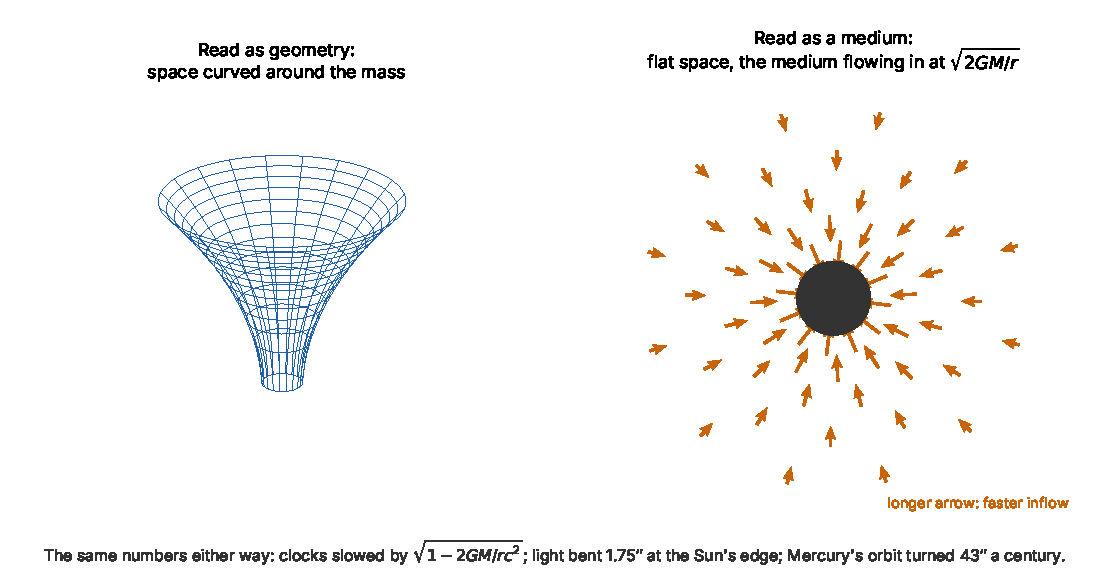
\includegraphics[width=\linewidth]{fig08-1-two-readings.pdf}
\caption{One set of numbers, two readings. Left: space curved around a mass, the picture usually drawn. Right: flat space, with a medium flowing in at the escape speed. The two give the same clock rates, the same bending of light and the same turning of orbits, because they are the same solution of general relativity's equations, written two ways.}\label{fig:readings}
\end{figure}

\argm{The geometry outside a mass can be read as a flow.} In 1921 and 1922 Painlev\'e and Gullstrand wrote the solution for the region outside a non-rotating mass in a form in which space is flat and something flows inward at the Newtonian escape speed, $\sqrt{2GM/r}$.\fn{painleve1921}\textsuperscript{,}\fn{gullstrand1922} Hamilton and Lisle developed it as the ``river model'' of black holes, extending it to spinning ones, where the river also turns.\fn{hamilton2008} Every number is the same: clocks, light, orbits, horizons (Figure~\ref{fig:readings}).

\argm{Matching numbers are not matching mechanisms.} When one solution can be read both as curved geometry and as a medium flowing in flat space, the numbers cannot decide which is what is there. That decision rests on mechanism: which reading names what touches what, and accounts for the energy. This is the Reduction Conflation of Part 3: agreement in numbers taken as agreement in what exists. In GPT \hypm{the river is the medium,} with clocks and rods slowed and squashed by the medium streaming through them, and its pressure lowered as it flows (Part 23).\fn{rashadaPart23} GPT keeps general relativity's numbers and supplies the ground they never had.

\section{Domain by Domain}

Each domain below sets out general relativity's account fairly, with its formula; where the account stops; GPT's mechanism; and what is measured. Table~\ref{tab:domains} summarises them.

\subsection{Orbits and the turning of Mercury}

\argm{General relativity's account:} the orbit equation gains a small term, $\dfrac{d^2u}{d\phi^2} + u = \dfrac{GM}{h^2} + \dfrac{3GM}{c^2}u^2$, with $u = 1/r$, and the extra term turns Mercury's ellipse by 43 arcseconds a century, as measured. It gives the number exactly and names no process.

\begin{hypbar}
\textbf{GPT's account: the sideways hold, weakened.} A planet's sideways motion holds it out against the inward acceleration of the medium. The medium's lowered pressure weakens that hold by the same factor that slows clocks: the radial motion obeys $(dr/d\tau)^2 = E^2 - (P/P_0)(c^2 + L^2/r^2)$. Near the Sun the hold is weaker, the planet swings in deeper and back later, and the orbit turns by $3\pi\,\Delta P/P_0$ each time round: 43.0 arcseconds a century for Mercury (Part 26).\footnotemark{}
\end{hypbar}
\footnotetext{\citealp{rashadaPart26}.}

\subsection{The rotation of galaxies}

\argm{General relativity's account,} with Newton's law as its limit, gives orbital speeds $v = \sqrt{GM(r)/r}$. The flat rotation curves of galaxies need more mass than is seen, and the standard account adds dark matter, fitted galaxy by galaxy; no particle of it has been detected. GPT's account is the relaxation boundary at $a_0$, set by the visible mass alone, with the measured relation in which every galaxy follows one curve (Part 9).\fn{rashadaPart9}

\subsection{Clocks}

\argm{General relativity's account:} a clock at distance $r$ runs at $\sqrt{1-2GM/rc^2}$ of the rate of one far away, and a moving clock is slowed by special relativity's factor; GPS corrects for both. Clocks slow, and the theory says by how much; it does not say what slows them.

\begin{hypbar}
\textbf{GPT's account: one effect.} A clock is slowed by the medium streaming past it, whether the streaming is the inflow or the clock's own motion: its rate is $\sqrt{P/P_0} = \sqrt{1-w^2/c^2}$. The height gain and the speed loss of a GPS clock are one effect, and give 38.5 microseconds a day with no fitted constant (Parts 9 and 10).\footnotemark{}
\end{hypbar}
\footnotetext{\citealp{rashadaPart10}.}

\subsection{The bending of light}

\argm{General relativity's account:} light passing a mass at distance $b$ is bent by $4GM/bc^2$, 1.75 arcseconds at the Sun's edge. It follows a geodesic of the curved geometry. But the standard account's own calculations of lensing use a refractive index, $n \approx 1 + 2GM/c^2r$: Eddington described the bending so in 1920, and the standard textbook on gravitational lenses derives the bending and the delay from it.\fn{eddington1920}\textsuperscript{,}\fn{schneider1992} In GPT \hypm{the index is the medium's,} raised where its pressure is lowered (Part 10). A refractive index is a property of a medium.

\subsection{The dragging of frames}

\argm{General relativity's account:} near a spinning mass the metric gains a term linking time and rotation, $g_{t\phi} \propto GJ\sin^2\theta/c^3r$, and a gyroscope's axis is turned. Gravity Probe B measured the turning around the Earth at $37\pm7$ milliarcseconds a year, against 39 predicted.\fn{everitt2011} What physically is being dragged? How does the rotation of a mass turn something in empty space? The theory says ``spacetime'' and stops.

\begin{hypbar}
\textbf{GPT's account: the medium's swirl.} A spinning mass sets the medium around it turning, strongest toward its equator, and the turning carries a gyroscope's axis with it (Part 16).\footnotemark{} It is not spacetime that twists, but the medium that swirls. GPT also expects a rotational imprint beyond what a body's shape gives, which general relativity does not, and which can be tested.
\end{hypbar}
\footnotetext{\citealp{rashadaPart16}.}

\subsection{Redshift}

\argm{General relativity's account:} light climbing from a source at $r_s$ to an observer at $r_o$ arrives with its frequency lowered by $\sqrt{(1-2GM/r_sc^2)/(1-2GM/r_oc^2)}$, the ratio of the clock rates at the two places. In GPT \hypm{the redshift is the difference between clocks:} the source's rhythm is slowed by the faster stream of the medium there, and the light carries that rhythm to where clocks run faster (Part 10).\fn{okun2000} The two agree in number. Measured redshifts are the same at every wavelength, as both require.

\subsection{Gravitational waves}

\argm{General relativity's account:} accelerating masses send out waves in the metric, travelling at the speed of light, with two transverse polarisations, carrying energy away.\fn{isaacson1968} All of this is measured. What is waving? The theory's answer is the metric: the geometry itself. A wave in something with no constitution is a metaphor, not a mechanism. In GPT \hypm{the waves are transverse waves of the medium,} carried at the speed its stiffness and inertia allow, as light is (Parts 15 and 28).\fn{rashadaPart28}

\begin{table}[t]\centering\small
\caption{Domain by domain: general relativity's account, where it stops, and GPT's mechanism. In every row both give the measured number.}
\begin{tabularx}{\linewidth}{@{}>{\raggedright}p{0.14\linewidth} >{\raggedright}p{0.24\linewidth} >{\raggedright}p{0.22\linewidth} X@{}}\toprule
\textbf{Domain} & \textbf{General relativity} & \textbf{Where it stops} & \textbf{GPT}\\\midrule
Orbits & extra term in the orbit equation & names no process & the medium's lowered pressure weakens the sideways hold\\
Galaxies & dark matter added & not detected & relaxation boundary at $a_0$\\
Clocks & rate $\sqrt{1-2GM/rc^2}$, and motion & what slows the clock & the medium streaming past, one effect\\
Light & geodesic; computed with an index & whose index & the medium's index\\
Frame dragging & the metric's rotation term & what is dragged & the medium's swirl\\
Redshift & ratio of clock rates & as for clocks & the difference between clocks\\
Waves & waves in the metric & what is waving & transverse waves of the medium\\
Energy & total conserved; not localizable & where the energy is & the medium's pressure, converted to flow\\\bottomrule
\end{tabularx}\label{tab:domains}\end{table}

\section{The Energy Ledger}

\argm{The ledger has gaps in the standard account.} For an isolated system, general relativity gives a total energy that is conserved, and the energy a binary loses to waves is computed and measured. But it gives no energy density for gravity at a place, only constructions that change with the choice of coordinates; and in the expanding universe, light loses energy to its redshift with nowhere stated for the energy to go. A body moving toward the Earth gains energy each second, and the theory says only that nothing acts on it.

\begin{hypbar}
\textbf{GPT's ledger: the medium pays, and the payment is located.}
\begin{itemize}
\item \textbf{A body moving toward the Earth} is carried by the medium, which delivers momentum to every particle in proportion to its mass, $mg$ every second. Its energy comes from the medium's pressure, converted into flow. Momentum is not merely observed; it is delivered (Parts 7 and 11).
\item \textbf{A body held} has the same momentum delivered and relays it into its support; the push appears only when the motion is stopped. Its weight is that push (Part 6).
\item \textbf{A body lifted} returns energy to the medium's pressure, and the medium returns it on the way down. ``Potential energy'' is the medium's pressure, located.
\item \textbf{An orbit} is a body coasting sideways through a medium that is itself accelerating inward. Nothing is paid to keep it going.
\end{itemize}
\end{hypbar}

\argm{Where general relativity bends coordinates, GPT maps flows.} Both keep the books balanced in total; GPT says where each entry is.

\section{Questions for Any Account of Gravity}

Five questions sharpen the difference. Each is put fairly: general relativity's answer as the theory gives it, what remains, and GPT's answer with its status.

\paragraph{1. What causes gravity?} General relativity: matter and energy determine the geometry, and bodies follow its geodesics. That says what happens, and how much; it does not say what matter does to the geometry or what the geometry does to the body. GPT: \hypm{the medium flows into every mass,} and every body in the flow is carried by it.

\paragraph{2. What is waving in a gravitational wave?} General relativity: the metric, the geometry of spacetime. That names a mathematical object, measured to carry energy, momentum and two polarisations at the speed of light. GPT: \hypm{the medium, in transverse waves.}

\paragraph{3. Where is the energy?} General relativity: conserved in total for an isolated system; not localizable. GPT: \hypm{in the medium's pressure,} converted to flow and back.

\paragraph{4. Why does the language of force remain?} General relativity: it is the weak-field approximation's convenience. But the approximation's convenience is also its explanation in practice: the word ``pull'' does the explaining, and names nothing (Part 7). GPT: \hypm{the force is the medium's delivery of momentum,} and the push appears where the motion is stopped.

\paragraph{5. What is spacetime, if it is real?} General relativity: a manifold with a metric; whether it exists as a thing is unsettled, and its founder said both that it lost its last physical objectivity and that it is endowed with physical qualities. GPT: \hypm{a medium,} with the properties general relativity already assigns it.

\section{The Break}

\argm{Where the two agree, and where they cannot.} General relativity and GPT can agree on every number: the river reading shows that one solution carries both. They cannot agree on what exists and what causes. General relativity says gravity is not a force, that nothing acts on a body moving freely, that the energy of gravity has no place, and, in the reading usually taught, that spacetime is not a substance. GPT says a medium is there, that it delivers momentum to every body it carries, that the energy is in its pressure, and that what general relativity calls spacetime has the properties of that medium. These are not two versions of the same claim. On what is there, only one can be right.

\argm{The standard account computes as if space were empty, and adds what space contains.} The universe of the standard account is five per cent ordinary matter; the rest is dark matter, never detected, and dark energy, whose nature is unknown.\fn{planck2018vi} When corrections outgrow what they correct, it is a sign the foundation is missing something (Part 14). GPT's proposal is that the missing thing is the medium general relativity already describes and does not name.

General relativity mapped the shape. GPT builds the structure.

\section*{Conclusion}
\addcontentsline{toc}{section}{Conclusion}

General relativity is a precise and well-tested description of how bodies and light move, and of how clocks run, near mass. Stated fairly, it does not borrow Newton, does not lack a field, does not require the geometric picture, and its author did not say that space is nothing. Its gap is elsewhere. Its two central statements are equalities, not mechanisms; its energy of gravity has no address; its language of force has no carrier. And it treats spacetime as real, giving it curvature, waves, energy, stiffness, rotation, expansion and a frame of rest, without saying what spacetime is. To identify it would require a local energy, a state of motion, an exchange with matter and a constitution; and anything with those is a medium. The same numbers read as a medium flowing in flat space show that the numbers cannot decide between geometry and medium; mechanism must. Domain by domain, GPT gives the mechanism for what general relativity describes. The break is philosophical before it is mathematical: not over what is measured, but over what is there.

\clearpage
\section*{Changes in the Second Edition}
\addcontentsline{toc}{section}{Changes in the Second Edition}

This list records what changed from the first edition and why. Changes to the argument alter what the paper claims or how it supports a claim; clarifications improve wording, sources or presentation and leave the argument as it was.

\subsection*{Changes to the argument}
\begin{itemize}
\item \textbf{The break is redefined.} The first edition called general relativity ``structurally incomplete and causally opaque'', said it ``collapses under scrutiny'', and called for its ``complete and irreversible'' replacement. The break is now located where it is: not in the numbers, which both accounts must give and which GPT reproduces (the river reading), but in what each says exists and causes. ``GPT as replacement'' becomes GPT keeping general relativity's numbers and supplying their ground.
\item \textbf{What general relativity says is stated fairly.} Corrected: that it relies on Newton (Newton's law is its weak-field limit, and the corrections are its own expansion); that it has no field and an inert background (the metric is a dynamical field); that it treats gravity as nonlocal (changes travel at $c$); that it cannot conserve energy (it conserves the total for isolated systems; it cannot localise gravitational energy). Added: the field-in-flat-spacetime route to the same equations (Feynman, Deser, Weinberg), and Einstein's 1920 statements on the ether.
\item \textbf{The reification of spacetime} is added as the central argument: what spacetime is given in the standard account, what identifying it as real would require, and what that would imply. The first edition's ``GR treats mathematical structure as physical cause'' and ``waves without a medium'' are kept within it.
\item \textbf{Orbits.} ``Comparable predictive accuracy'' from ``pressure distributions and resonant dynamics'', $F = -\nabla P_g$, and the orbital speed $v = \sqrt{r\nabla P_g/\rho}$ are replaced by the weakened sideways hold, giving 43.0 arcseconds a century (Part 26).
\item \textbf{Galaxies.} ``Structured graviton flow asymmetry'' is replaced by the relaxation boundary at $a_0$ (Part 9).
\item \textbf{Clocks.} The law $d\tau/dt = \sqrt{P_0/P}$ is inverted in the first edition and is corrected to $\sqrt{P/P_0}$. ``Coherence-based time modulation'', reported as demonstrated, is withdrawn: no such measurement exists, and every kind of clock tested slows by the same factor.
\item \textbf{Light.} The index $n_g \propto \sqrt{P_g}$ is replaced by $n = P_0/P$. Proposed instruments to detect ``graviton density fields'' are removed.
\item \textbf{Frame dragging.} The formula $\vec F = -\nabla P_g + \vec v_r \times (\nabla\times\vec P_g)$, whose terms do not have the units of force, is withdrawn; frame dragging is the medium's swirl (Part 16). ``Frequency-dependent'' frame dragging is withdrawn. The first edition's questions (what is dragged; how rotation alters empty space) are kept.
\item \textbf{Redshift.} ``Pressure band tuning'', frequency-dependent and polarisation-dependent redshift are withdrawn: measured redshifts are the same at every wavelength. The redshift is the difference between clocks (Part 10).
\item \textbf{The energy ledger.} ``The apple is pushed from above'' is replaced by the medium carrying the body (Part 7); ``orbit as pressure equilibrium'' by coasting through an accelerating medium; ``the illusion of spacetime locality'' is withdrawn, since general relativity is local.
\item \textbf{The five questions} are kept, with general relativity's answers stated as it gives them. Question 4 becomes why the language of force remains; question 5, on coherence and structure, becomes what spacetime is, if it is real.
\item \textbf{Removed:} gravitational shielding, propulsion and ``architectural resonance'' technologies; coherence-tuned shielding; ``engineered gravitational technologies''. Shielding is bounded far below what these need (Part 15).
\end{itemize}

\subsection*{Clarifications}
\begin{itemize}
\item The tone is changed: ``showdown'', ``illusion'', ``ideological enclosure'', ``paradigm in decline'', ``narration is not science'' and similar phrases are removed. The comparisons are kept, domain by domain, in Table 8.2.
\item The subtitle changes from \textit{Exposing the Irreconcilable Contradictions} to \textit{The Irreconcilable Differences}.
\item One figure and two tables are added; sources are added for each statement about general relativity.
\end{itemize}

\bibliography{part08}
\end{document}
